\documentclass{article}
\title{Senior Projects Holography Report}
\date{2018-12-02}
\author{Ben Sterling, Dongkyu Kim, Junbum Kim, David Kim}

\usepackage{amsmath}
\usepackage{mathrsfs}
\usepackage[pdftex]{graphicx}

\begin{document}
\maketitle
\clearpage

\section{Introduction}

The objective of the project is to create a 3D sample of a real-life object and project onto a surface as a hologram. The applications of this project include displaying an artwork or a building schematic in 3D to help visualize the product for artists and architects. We believe this is a great alternative to existing solutions as the previous technologies are difficult and time consuming. Several prototyping tools and techniques exist including AutoCAD, SolidWorks, and 3D printing. The AutoCAD and SolidWorks are programs that require the user to manually model the real life object, and 3D printing also requires a model that has been already modeled digitally. In addition, 3D printing often takes a while to create a 3D object in real life depending on the size of the object. The substages of the projects can be largely divided into include the sampling stage, digital conversion stage, digital projection stage, and optical holography projection stage. The following report discusses each step in more detail.

\section{Sampling Stage}

As the focus of the project was to investigate holographic application, existing solutions for 3D reconstruction tools were used for the project. Xbox Kinect for Windows Development was the specific machine used for the project. Windows Presentation Foundation (WPF) application was built to communicate the hardware with software. Kinect Studio Version 2.0 and Kinect Software Development Kits were installed to develop the program. Specifically, the KinectFusionExplorer module proved practical for the purpose. The module allows 3D modelling from a single photo shoot from one angle by reconstructing picture from plain camera, infrared sensors, and depth sensors. Although the technology cannot provide a 360-degree capture of the sample, it does reconstruct the sides of the image with only small depth errors. The rotation of the model allows users to see the sides of the real object within the computer. Note that USB 3.0 is required to reproduce the program, as the Kinect hardware requires the extra bandwidth for communication of data. 

\section{Digital Conversion Stage}

Bitmaps can be constructed from the 3D model constructed, but the exact input for source light modulator has not exactly been specified yet, and since the development of the digital conversion stage basically depends on the exact requirement of SLM, this field has yet not been developed properly yet.

\section{Digital Projection Stage}

SLM is simply speaking, a monitor. It takes a digital output from servers via an HDMI cable. Python programs will run on top of the WPF application to project data onto SLM via wireless HDMI. Modules such as slmpy exist to perform SLM projection. This is yet a step being investigated.

\section{Holography Background}

\subsection{Wave Fundamentals}

The fundamentals of Holography start from Maxwell's Equations. In the most general case, they are formulated as follows:

\begin{equation}
	\nabla \cdot \vec{D} = \rho\\
\end{equation}

\begin{equation}
	\nabla \cdot \vec{B} = 0
\end{equation}

\begin{equation}
	\nabla \times \vec{H} = \vec{J} + \frac{\partial \vec{D}}{\partial t}
\end{equation}

\begin{equation}
	\nabla \times \vec{E} = -\frac{\partial \vec{B}}{\partial t}
\end{equation}

However, we are interested in utilizing these equations to study optics. Since light waves travel in the air, \(\rho\) = 0 and \(\vec{J}\) = \(\vec{0}\) because there is no source charge or current in the air. Here are the equations we obtain setting sources to zero:

\begin{equation}
	\nabla \cdot \vec{D} = 0
\end{equation}

\begin{equation}
	\nabla \cdot \vec{B} = 0
\end{equation}

\begin{equation}
	\nabla \times \vec{H} = \frac{\partial \vec{D}}{\partial t}
\end{equation}

\begin{equation}
	\nabla \times \vec{E} = -\frac{\partial \vec{B}}{\partial t}
\end{equation}

Lastly, we want to relate D to E, and B to H. The most general relationships that describes these quantities are:

\begin{equation}
	\vec{D} = \epsilon_{0}\vec{E} + \vec{P}
\end{equation}

\begin{equation}
	\vec{B} = \mu_{0}(\vec{H} + \vec{M})
\end{equation}

We assume that all the materials we are working in are Linear, Homogeneous, and Isotropic. The last two equations can be simplified to:

\begin{equation}
	\vec{D} = \epsilon\vec{E}
\end{equation}

\begin{equation}
	\vec{B} = \mu\vec{H}
\end{equation}

where \(\epsilon\) = \(\epsilon_{r}\)\(\epsilon_{0}\) and \(\mu\) = \(\mu_{r}\)\(\mu_{0}\) are constants. If we combine the last two equations along with Maxwell's Equations we get:

\begin{equation}
	\nabla \cdot \vec{E} = 0
\end{equation}

\begin{equation}
	\nabla \cdot \vec{H} = 0
\end{equation}

\begin{equation}
	\nabla \times \vec{H} = \epsilon\frac{\partial E}{\partial t}
\end{equation}

\begin{equation}
	\nabla \times \vec{E} = -\mu\frac{\partial H}{\partial t}
\end{equation}

then we utilize the following identity from vector calculus:

\begin{equation}
	\nabla^2F = \nabla(\nabla \cdot F) - \nabla\times\nabla\times F
\end{equation}

and get:

\begin{equation}
	\nabla^2E - \mu\epsilon\frac{\partial^2 E}{\partial t^2} = 0
\end{equation}

\begin{equation}
	\nabla^2H - \mu\epsilon\frac{\partial^2 H}{\partial t^2} = 0
\end{equation}

The Multi-Dimensional Fourier Transform is defined as follows:

\begin{equation}
	\hat{f} (\vec{k}) = \iint \limits_{R^n}^{} f(\vec{x})e^{-j \vec{k} \cdot \vec{x}} \,d\vec{x}
\end{equation}

and a plane wave is defined as follows:

\begin{equation}
	\vec{E} = \vec{E_{0}}e^{j \omega t - j\vec{k} \cdot \vec{x}} 
\end{equation}

Because E and H field are functions of x, y, z, and time, it is possible to span all E and H fields with a superposition of plane waves. This motivates the notation:

\begin{equation}
	\vec{E} = \vec{E_{0}}\psi
\end{equation}

where

\begin{equation}
	\psi = e^{j \omega t - j\vec{k} \cdot \vec{x}}
\end{equation}

Thus, in \(\psi\) notation, the wave equation turns into:

\begin{equation}
	\nabla^2\psi - \mu\epsilon\frac{\partial^2\psi}{\partial t^2} = 0
\end{equation}

\subsection{Plane and Spherical Wave Applications}

For a single frequency, we are interested in the complex amplitude, \(\psi_{p}\) we define as follows:

\begin{equation}
	\psi = \psi_{p}e^{j \omega t}
\end{equation}

We can think of this quantity like the phasor representation of \(\psi\).

The central application of the classical theory is to develop the math behind Fresnel Diffraction. An aperture can be visualized by this diagram:
\begin{center}
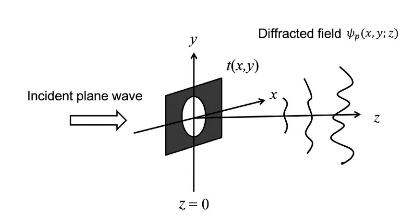
\includegraphics[width=100mm]{tupac5.png}
\end{center}

We also define \(k_{0}\) as the wave number in free space, such that

\begin{equation}
	\nabla^2\psi_{p} + k_{0}^2\psi_{p} = 0
\end{equation}

since

\begin{equation}
	\lambda f = c \rightarrow k_{0} = \omega/c
\end{equation}

By considering the incoming plane wave as a superposition of plane waves (like we did with the Multi-Dimensional Fourier Transform), we obtain the result:

\begin{equation}
	\mathscr{F} \Big\{ \frac{\partial^2 \psi_{p}}{\partial x^2} \Big\} = (-jk_{x})^2\Psi_{p} = -k_{x}^2\Psi_{p}
\end{equation}

and

\begin{equation}
	\mathscr{F} \Big\{ \frac{\partial^2 \psi_{p}}{\partial y^2} \Big\} = (-jk_{y})^2\Psi_{p} = -k_{y}^2\Psi_{p}
\end{equation}

where 

\begin{equation}
	\Psi_{p} = \mathscr{F} \{\psi_{p}\}
\end{equation}

Finally, if we take the Fourier Transform of both sides of (26) we obtain:

\begin{equation}
	\frac{\partial^2\Psi_{p}}{\partial z^2} + k_{0}^{2} \bigg ( 1 - \frac{k_{x}^2}{k_{0}^2} - \frac{k_{y}^2}{k_{0}^2} \bigg ) \Psi_{p} = 0
\end{equation}

While this looks complicated, it is really only an Ordinary Differential Equation of \(\Psi_{p}\) with respect to z. It's solution is:

\begin{equation}
	\Psi_{p} = \big(\Psi_{p}\vert_{z = 0}\big) exp\bigg(-jk_{0}z\sqrt{1 - \frac{k_{x}^2}{k_{0}^2} - \frac{k_{y}^2}{k_{0}^2}}\bigg)
\end{equation}

If we let

\begin{equation}
	\Psi_{p0} = \big(\Psi_{p}\vert_{z = 0}\big)
\end{equation}

Then we can recognize the solution in (32) as a transfer function. We define:

\begin{equation}
	\mathscr{H} = \frac{\Psi_{p}}{\Psi_{p0}} = exp\bigg(-jk_{0}z\sqrt{1 - \frac{k_{x}^2}{k_{0}^2} - \frac{k_{y}^2}{k_{0}^2}}\bigg)
\end{equation}

\(\mathscr{H}\) is called the Spatial Frequency Transfer Function of Propagation. It applies to our specific apparatus under consideration and describes Fresnel Diffraction of the output of a plane wave hitting an aperture. \(\psi_{p0}\) is the function controlled by the shape of the aperture; if this equals \(\delta(x,y)\), for example, then the output of the aperture is purely the Spatial Frequency Transfer Function response, because this is equivalent to convolving with a delta in 2-Dimensions, returning \(\mathscr{F}^{-1} \{\mathscr{H}\} \) in the time domain.

\subsection{Holography Fundamentals}

\subsubsection{Holgraphic Magnifications}
\subsubsection{Holographic Translation}
\subsubsection{Holographic Magnification}

\subsection{Types of Holograms}
\subsubsection{On-Axis Holography}
\subsubsection{Off-Axis Holography}

\section{Project Setup}

\begin{center}
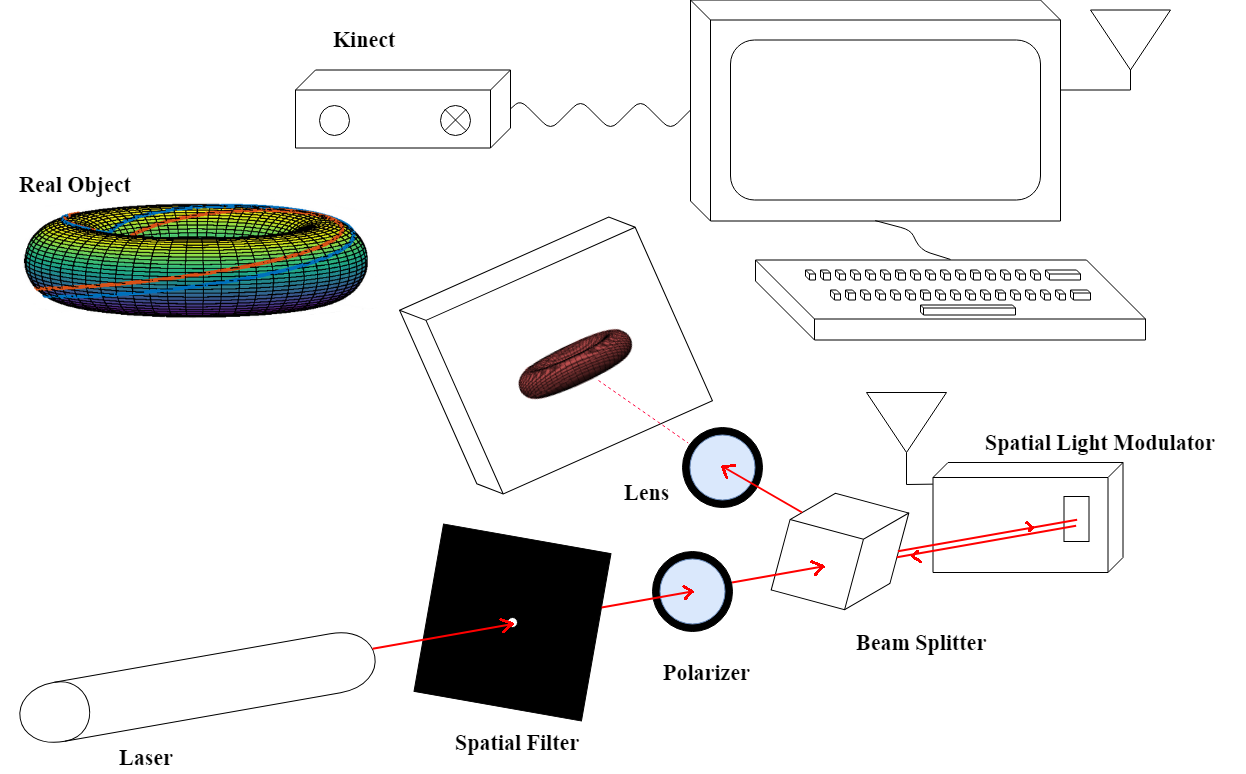
\includegraphics[width=100mm]{tupac10.png}
\end{center}

\section{List of Materials}

\section{What we have done}

\section{Future goals}

\end{document}
